\documentclass[11pt,a4paper]{article}

\usepackage[utf8]{inputenc}
\usepackage[T1]{fontenc}
\usepackage[italian]{babel}
\usepackage{lmodern}
\usepackage[margin=2.2cm]{geometry}
\usepackage{booktabs}
\usepackage{graphicx}
\usepackage{xcolor}
\usepackage{enumitem}
\usepackage{amssymb}
\usepackage[hidelinks]{hyperref}

\newcommand{\cfg}[1]{\texttt{#1}}
\setlist{itemsep=2pt}

\title{Report finale -- Modelli DfpNet Mamba e tuning}
\author{}
\date{18/10/2026 \\ \small Fonte: \texttt{train/metrics/}}

\begin{document}
\maketitle

\section*{Sintesi}

Il modello migliore è \textbf{HalfMamba\_Augmented, Combination 4}: Mamba 16-2-4 su \cfg{out1}, \cfg{out2} e \cfg{out2b}, più un blocco \textbf{32-2-4} nel decoder a $64\times64$. Ha un errore di validazione dell'\textbf{1,628\%} ($-16{,}8\%$ rispetto alla baseline) con il \textbf{+10,5\% di parametri} e 30\,s per epoca.

\begin{itemize}
  \item \textbf{Miglior compromesso:} Combination 12 (\cfg{out2} a 24-2-2). Errore 1,673\% ($-14{,}5\%$), +9,8\% di parametri, 27,4\,s per epoca.
  \item \textbf{Massima efficienza:} \cfg{M\_out1}, un solo blocco Mamba a $64\times64$. Dà $-8{,}7\%$ con appena +1,2\% di parametri e 15,8\,s per epoca.
  \item \textbf{Il tuning conta soprattutto nel decoder e su \cfg{out2}.} Toccare \cfg{out1} non migliora mai il riferimento, e \cfg{out2b} a 32-2-2 è la scelta peggiore.
  \item \textbf{Limite:} tutte le run sono a 1 seed, e lo stesso modello cambia fino a 0,15 punti tra il seed 34 e il 42. Le differenze sotto $\sim$0,1 punti non sono affidabili.
\end{itemize}

\section{Metodologia}

Tutti i modelli sono confrontati con la stessa metrica, ricalcolata dai file \cfg{metrics\_train.csv} di ogni run in \cfg{train/metrics/}.

\begin{itemize}
  \item \textbf{Errore val (20):} media di \cfg{val\_rel\_error} nelle ultime 20 epoche su 150. È la metrica già usata da \cfg{runTuning.py} ed è più stabile dell'ultima epoca.
  \item \textbf{Baseline:} media dei 3 seed (42, 1955, 2003) $= \mathbf{1{,}958\% \pm 0{,}025}$. \cfg{runTuning.py} usa invece 1,953\%, cioè il solo seed 42, quindi i suoi ``improvement'' sono leggermente diversi da quelli qui.
  \item \textbf{$\Delta$ parametri:} rispetto ai 2.332.035 parametri della baseline (\cfg{expo = 5}), contati con il codice attuale di \cfg{DfpNet.py}. Per le run storiche allenate con codice vecchio (es.\ \cfg{mambaSup} con \cfg{ssm\_conv = 3}) il conteggio è approssimato.
  \item \textbf{Tempo e VRAM:} media dall'epoca 2 in poi. La baseline non li ha registrati. Come riferimento uso i $\sim$10,4\,s per epoca dei modelli con attention a bassa risoluzione (\cfg{A\_out2}\dots\cfg{A\_out5}), che costano quasi quanto la baseline.
  \item \textbf{Riferimento del tuning:} \cfg{HMdec\_d2}, cioè la stessa architettura di HalfMamba\_Augmented con tutti i blocchi a 16-2-4 e lo stesso seed 42. Errore 1,733\%.
  \item \textbf{Esclusa:} la run \cfg{HalfMamba\_Augmented\_Combination\_\{i\}\_s42} (1,686\%). Il nome viene da un bug del vecchio script e non si sa quale configurazione abbia usato.
\end{itemize}

\section{Panoramica di tutti i modelli}

Sono stati provati 33 modelli fuori dal tuning: 24 riducono l'errore della baseline di più del 3\%, e tutti i 14 migliori hanno Mamba a \cfg{out1} ($64\times64$). M = blocco Mamba 16-2-4, m = Mamba small, A = self-attention. $\Delta$ errore negativo = meglio della baseline. Le 15 combinazioni del tuning sono nella Sezione~\ref{sec:tuning}.

\begin{table}[h!]
\centering
\caption{Risultati di validazione di tutti i modelli (ordinati per errore).}
\label{tab:tutti}
\resizebox{\textwidth}{!}{%
\begin{tabular}{@{}lllrrrrrr@{}}
\toprule
Modello & Mixer & Seed & Errore val (20) & $\Delta$ errore & Parametri & $\Delta$ param. & s/epoca & VRAM MB \\
\midrule
\cfg{HMdec\_d2} & halfMamba + dout2 & 42 & 1,733\% & $-11{,}5\%$ & 2,56\,M & +10,0\% & 27,0 & 723 \\
\cfg{HMdec\_d2\_d2b} & halfMamba + dout2, dout2b & 42 & 1,739\% & $-11{,}1\%$ & 2,65\,M & +13,8\% & 30,5 & 815 \\
\cfg{HMdec\_d2\_d2b\_d3} & halfMamba + dout2, dout2b, dout3 & 42 & 1,750\% & $-10{,}6\%$ & 2,74\,M & +17,5\% & 32,0 & 840 \\
\cfg{halfMamba\_lightconv1} & M out1, out2, out2b & 42 & 1,753\% & $-10{,}5\%$ & 2,54\,M & +8,8\% & 23,4 & 501 \\
\cfg{MMM\_AA} & M out1--out2b; A out4, out5 & 42 & 1,761\% & $-10{,}0\%$ & 3,06\,M & +31,4\% & 25,4 & 527 \\
\cfg{halfMamba} & M out1, out2, out2b & 42 & 1,777\% & $-9{,}2\%$ & 2,54\,M & +8,8\% & 23,9 & 506 \\
\cfg{M\_out1} & M out1 & 42 & 1,788\% & $-8{,}7\%$ & 2,36\,M & +1,2\% & 15,8 & 385 \\
\cfg{halfMambaPush} & M out1, out2; A out2b & 42 & 1,789\% & $-8{,}6\%$ & 2,47\,M & +5,7\% & 21,4 & 415 \\
\cfg{MambaMentality\_convo} & M in, out1--out2b & 42 & 1,795\% & $-8{,}3\%$ & 2,54\,M & +8,9\% & 34,3 & 729 \\
\cfg{MM\_\_\_\_} & M out1, out2 & 42 & 1,800\% & $-8{,}1\%$ & 2,45\,M & +5,0\% & 19,1 & 479 \\
\cfg{Mmm\_\_\_} & M out1; m out2, out2b & 42 & 1,813\% & $-7{,}4\%$ & 2,44\,M & +4,5\% & 22,3 & 446 \\
\cfg{MMAA\_\_} & M out1, out2; A out2b, out3 & 42 & 1,820\% & $-7{,}0\%$ & 2,53\,M & +8,6\% & 22,8 & 497 \\
\cfg{fullMamba} & M out1, out2; m out2b--out5 & 42 & 1,822\% & $-6{,}9\%$ & 3,66\,M & +57,1\% & 35,3 & 515 \\
\cfg{halfMambaPush\_Light} & M out1, out2; A out2b & 42 & 1,828\% & $-6{,}6\%$ & 2,47\,M & +5,7\% & 20,2 & 409 \\
\cfg{A\_out2} & A out2 & 42 & 1,859\% & $-5{,}0\%$ & 2,35\,M & +0,7\% & 10,5 & 207 \\
\cfg{A\_out1} & A out1 & 42 & 1,870\% & $-4{,}5\%$ & 2,34\,M & +0,2\% & 105,5 & 10324 \\
\cfg{M\_out2} & M out2 & 42 & 1,876\% & $-4{,}2\%$ & 2,42\,M & +3,8\% & 13,0 & 270 \\
\cfg{HalfMamba\_Augmented\_exp1} & M out1--out2b + dout2 & 34 & 1,881\% & $-3{,}9\%$ & 2,56\,M & +10,0\% & 27,3 & 676 \\
\cfg{M\_out3} & M out3 & 42 & 1,882\% & $-3{,}9\%$ & 2,63\,M & +12,8\% & 12,8 & 205 \\
\cfg{M\_out5} & M out5 & 42 & 1,882\% & $-3{,}8\%$ & 3,42\,M & +46,7\% & 12,8 & 210 \\
\cfg{M\_out2b} & M out2b & 42 & 1,886\% & $-3{,}6\%$ & 2,42\,M & +3,8\% & 12,8 & 201 \\
\cfg{MMMA\_\_} & M out1--out2b; A out3 & 42 & 1,889\% & $-3{,}5\%$ & 2,60\,M & +11,6\% & 25,1 & 517 \\
\cfg{A\_out3} & A out3 & 42 & 1,896\% & $-3{,}2\%$ & 2,40\,M & +2,8\% & 10,3 & 209 \\
\cfg{HalfMamba\_Augmented\_h24r2mlp6d} & M out1--out2b + dout2 & 34 & 1,896\% & $-3{,}2\%$ & 2,56\,M & +10,0\% & 28,5 & 751 \\
\cfg{A\_out2b} & A out2b & 42 & 1,906\% & $-2{,}6\%$ & 2,35\,M & +0,7\% & 10,4 & 195 \\
\cfg{MambaHead} & M huge out1; M out2, out2b & 34 & 1,911\% & $-2{,}4\%$ & 2,59\,M & +11,0\% & 30,9 & 676 \\
\cfg{MambaMentality} & M in, out1--out2b & 34 & 1,915\% & $-2{,}2\%$ & 2,54\,M & +8,9\% & 33,2 & 728 \\
\cfg{M\_out4} & M out4 & 42 & 1,920\% & $-1{,}9\%$ & 3,42\,M & +46,7\% & 13,0 & 126 \\
\cfg{A\_out4} & A out4 & 42 & 1,927\% & $-1{,}6\%$ & 2,60\,M & +11,3\% & 10,5 & 210 \\
\cfg{A\_out5} & A out5 & 42 & 1,932\% & $-1{,}3\%$ & 2,60\,M & +11,3\% & 10,4 & 208 \\
\cfg{mambaSup} & M out2b & 3 seed & 1,933\% $\pm$ 0,057 & $-1{,}3\%$ & 2,42\,M & +3,8\% & -- & -- \\
\textbf{\cfg{baseline}} & nessuno & 3 seed & 1,958\% $\pm$ 0,025 & -- & 2,33\,M & -- & -- & -- \\
\cfg{M1M3} & M out1, out2b & 34 & 2,044\% & $+4{,}4\%$ & 2,45\,M & +5,0\% & 19,5 & 408 \\
\bottomrule
\end{tabular}}
\end{table}

I 5 modelli allenati con il seed 34 stanno tutti nella metà bassa della classifica. HalfMamba\_Augmented ha la stessa architettura di \cfg{HMdec\_d2}, ma con il seed 34 fa 1,881\% invece di 1,733\%. Questa differenza da sola (0,15 punti) è più grande di quella che separa i primi 14 modelli.

\section{Migliori modelli}

Aggiungere parametri non basta: a parità di +10\% di parametri l'errore va dal $-3{,}9\%$ al $-16{,}8\%$. Quello che conta è dove si mette Mamba e come è configurato. Sono i migliori i modelli sulla linea blu della Figura~\ref{fig:params}, perché nessun altro modello fa meglio con meno parametri.

\begin{figure}[h!]
\centering
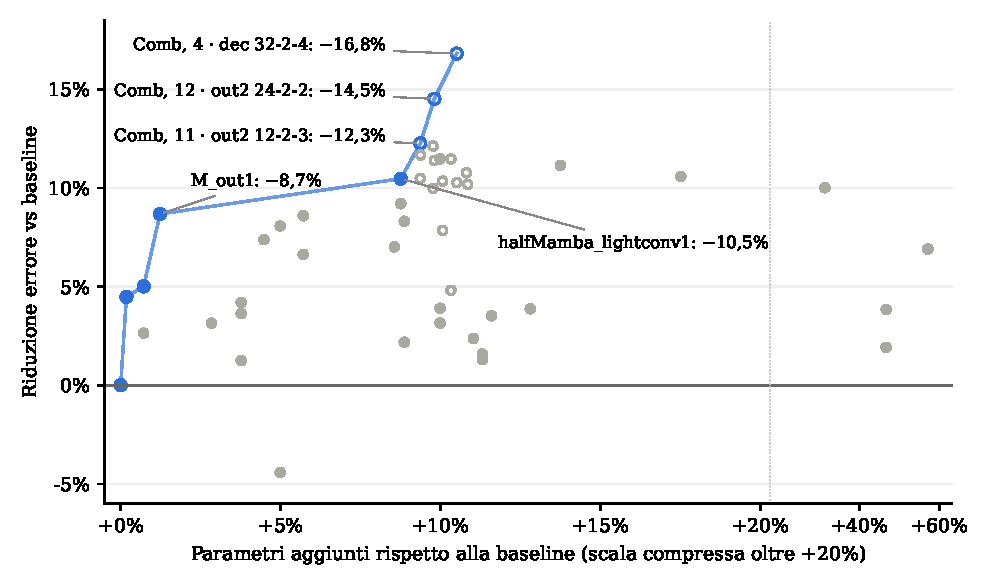
\includegraphics[width=\textwidth]{resources/report_finale/params_vs_errore.pdf}
\caption{Combination 4 riduce l'errore del 16,8\% con il 10,5\% di parametri in più. Riduzione dell'errore di validazione rispetto alla baseline per ogni modello. La linea blu unisce i modelli non dominati. Cerchi pieni: architetture provate. Cerchi vuoti: combinazioni del tuning di HalfMamba\_Augmented.}
\label{fig:params}
\end{figure}

\begin{table}[h!]
\centering
\caption{I quattro modelli migliori secondo prestazioni, parametri e tempo.}
\resizebox{\textwidth}{!}{%
\begin{tabular}{@{}rlllrrr@{}}
\toprule
\# & Modello & Perché & Errore val (20) & $\Delta$ param. & s/epoca & VRAM MB \\
\midrule
1 & Combination 4 & Miglior errore in assoluto & 1,628\% ($-16{,}8\%$) & +10,5\% & 30,0 & 744 \\
2 & Combination 12 & Miglior compromesso & 1,673\% ($-14{,}5\%$) & +9,8\% & 27,4 & 722 \\
3 & \cfg{M\_out1} & Miglior guadagno per parametro & 1,788\% ($-8{,}7\%$) & +1,2\% & 15,8 & 385 \\
4 & \cfg{halfMamba\_lightconv1} & Il più veloce tra quelli sopra il $-10\%$ & 1,753\% ($-10{,}5\%$) & +8,8\% & 23,4 & 501 \\
\bottomrule
\end{tabular}}
\end{table}

\begin{itemize}
  \item \textbf{Combination 4} è il migliore perché rinforza il blocco Mamba del decoder a $64\times64$ (\cfg{d\_state} da 16 a 32), dove la rete ricostruisce la scia. È l'unico modello che abbassa in modo visibile anche la pressione: 8,80\% contro il 9,70\% della baseline (circa 1,5 deviazioni standard). Il costo è circa 3 volte il tempo della baseline (30\,s contro $\sim$10\,s).
  \item \textbf{Combination 12} perde solo 0,045 punti rispetto alla 4, ma ha meno parametri, è il 9\% più veloce e usa 22\,MB in meno. È la scelta giusta se il tempo di training conta.
  \item \textbf{\cfg{M\_out1}} ottiene metà del guadagno della Combination 4 con un decimo dei parametri aggiunti (+28.576) e metà del tempo. Rende circa 7 punti di riduzione dell'errore per ogni 1\% di parametri, contro 1,6 della Combination 4.
  \item \textbf{\cfg{halfMamba\_lightconv1}} è il punto di partenza dei modelli successivi. Aggiungere il blocco del decoder (\cfg{HMdec\_d2}) costa +1,2\% di parametri e +3,6\,s per epoca per un punto in più di miglioramento.
\end{itemize}

\paragraph{Da evitare.} \cfg{fullMamba} (+57\% di parametri, 35\,s/epoca, solo $-6{,}9\%$), \cfg{MMM\_AA} (+31\% per lo stesso risultato di halfMamba), \cfg{M\_out4} e \cfg{M\_out5} (+47\% per $-2/-4\%$), \cfg{A\_out1} (105\,s/epoca e 10,3\,GB per $-4{,}5\%$). Anche altri blocchi nel decoder (\cfg{HMdec\_d2\_d2b}, \cfg{\_d3}) aggiungono fino al 17,5\% di parametri e 5\,s/epoca senza migliorare.

\section{Tuning degli iperparametri Mamba}
\label{sec:tuning}

Su 15 combinazioni solo 2 migliorano il riferimento in modo chiaro: il decoder a 32-2-4 ($-0{,}105$ punti) e \cfg{out2} a 24-2-2 ($-0{,}060$). Ogni configurazione è scritta come \cfg{d\_state}-\cfg{ssm\_ratio}-\cfg{mlp\_ratio}, e ogni combinazione cambia un solo blocco rispetto a 16-2-4.

\begin{figure}[h!]
\centering
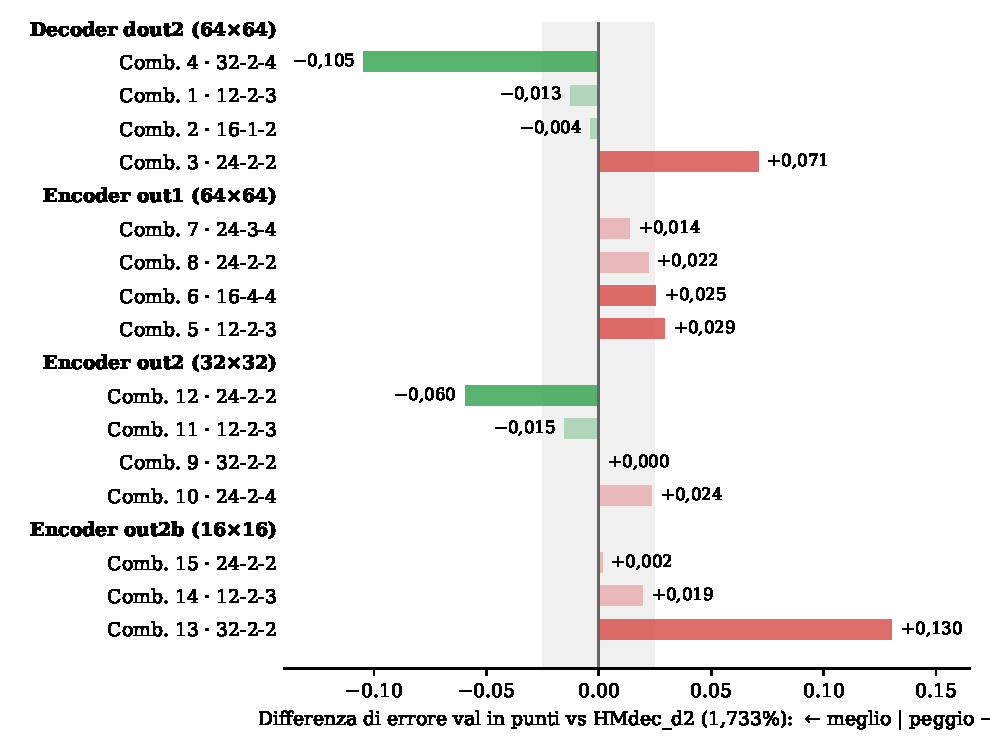
\includegraphics[width=\textwidth]{resources/report_finale/tuning_delta.pdf}
\caption{Solo due modifiche battono il riferimento oltre il rumore. Differenza dell'errore di validazione in punti rispetto a \cfg{HMdec\_d2} (tutti i blocchi 16-2-4, seed 42). Fascia grigia: $\pm1$ deviazione standard della baseline tra seed. Barre chiare: differenza dentro la fascia di rumore.}
\label{fig:tuning}
\end{figure}

\begin{itemize}
  \item \textbf{Decoder \cfg{dout2}: è il blocco più sensibile} (0,18 punti tra il migliore e il peggiore). Alzare \cfg{d\_state} a 32 tenendo \cfg{mlp\_ratio} 4 dà il miglior risultato di tutto il progetto. Con \cfg{mlp\_ratio} 2 (24-2-2) invece peggiora, quindi qui l'MLP serve. Il 16-1-2 resta pari al riferimento ma è il più leggero: 24,9\,s/epoca e 559\,MB di VRAM.
  \item \textbf{Encoder \cfg{out1}: qualsiasi modifica peggiora} (da +0,014 a +0,029). Le varianti più grandi costano anche di più: 16-4-4 arriva a 31,6\,s e 859\,MB. Va lasciato a 16-2-4.
  \item \textbf{Encoder \cfg{out2}: conviene ridurre l'MLP.} 24-2-2 e 12-2-3 migliorano con meno parametri, mentre 24-2-4 peggiora.
  \item \textbf{Encoder \cfg{out2b}: \cfg{d\_state} alto fa male.} Con 32-2-2 si ha il risultato peggiore del tuning (+0,130). A $16\times16$ la sequenza è di soli 256 token e uno stato grande non serve. 24-2-2 è neutro.
\end{itemize}

Due cose sono comuni a tutto il tuning. Il guadagno arriva dal ritoccare singoli blocchi, non dall'aumentare la capacità: tutte le combinazioni hanno tra +9,4\% e +10,9\% di parametri. E le differenze sotto $\sim$0,03 punti non vanno lette come effetti reali.

\section{Configurazione consigliata}

La configurazione che consiglio è la \textbf{Combination 4: 16-2-4 / 16-2-4 / 16-2-4 / 32-2-4} (\cfg{out1} / \cfg{out2} / \cfg{out2b} / decoder). La prossima run dovrebbe però provare a unirla alla Combination 12.

\begin{table}[h!]
\centering
\begin{tabular}{@{}lrrr@{}}
\toprule
Criterio & Combination 4 & Combination 12 & Riferimento (tutti 16-2-4) \\
\midrule
Errore val (20) & \textbf{1,628\%} & 1,673\% & 1,733\% \\
$\Delta$ vs baseline & $\mathbf{-16{,}8\%}$ & $-14{,}5\%$ & $-11{,}5\%$ \\
Errore pressione $p$ & \textbf{8,80\%} & 9,11\% & 9,29\% \\
$\Delta$ parametri & +10,5\% & \textbf{+9,8\%} & +10,0\% \\
Tempo per epoca & 30,0\,s & 27,4\,s & \textbf{27,0\,s} \\
VRAM & 744\,MB & \textbf{722\,MB} & 723\,MB \\
\bottomrule
\end{tabular}
\end{table}

\noindent Perché la Combination 4:
\begin{itemize}
  \item \textbf{Prestazioni:} è la migliore su tutte e tre le componenti ($p$, $v_x$, $v_y$). Il guadagno sul riferimento (0,105 punti) è circa 4 volte la deviazione standard della baseline tra seed.
  \item \textbf{Parametri:} costa solo lo 0,5\% in più del riferimento. Rispetta il vincolo di iso-capacità come tutti i modelli halfMamba.
  \item \textbf{Tempo:} +3\,s per epoca (+11\%), cioè circa 7 minuti in più su 150 epoche. È un costo piccolo per il miglior risultato del progetto.
\end{itemize}

Se conta di più il tempo, la Combination 12 dà l'86\% del guadagno ed è la più economica tra le migliori. Se contano soprattutto i parametri, resta \cfg{M\_out1}.

\subsection*{Passi successivi}
\begin{itemize}[label=$\square$]
  \item Allenare la combinazione unita \textbf{16-2-4 / 24-2-2 / 16-2-4 / 32-2-4}. Le due modifiche toccano blocchi diversi e potrebbero sommarsi (circa +10,3\% di parametri).
  \item Rilanciare Combination 4, Combination 12 e la combinazione unita con 3 seed (42, 1955, 2003). Con un solo seed lo stesso modello oscilla fino a 0,15 punti.
  \item Provare \cfg{d\_state} 48 o 64 sul decoder: è l'unico blocco in cui alzare \cfg{d\_state} ha aiutato.
  \item Valutare i modelli finali sul test set con \cfg{runTest.py}. Oggi solo la baseline ha un risultato sul test.
  \item Registrare tempo e VRAM della baseline, per confrontare i costi in modo diretto.
\end{itemize}

\end{document}
